\subsubsection{Analog Frontend Design}

\paragraph{Analog Input Stage Design}

\subparagraph{Input AC Coupling}
\label{sec:input-ac-coupling}

The TLV320AIC series codec has a configurable input impedance of \qty{10}{\kilo\ohm}, \qty{20}{\kilo\ohm}, and \qty{40}{\kilo\ohm} \cite{TLV320AIC3204ApplicationReference2012}.
To achieve the lowest possible high-pass cutoff frequency with a given coupling capacitor, the maximum input impedance of \qty{40}{\kilo\ohm} is selected.


The AC-coupling capacitor together with the input impedance of the codec ADC forms a simple RC high-pass filter, whose cutoff frequency is given by:
\[
f_c = \frac{1}{2 \pi R_\text{eq} C_c}
\]
The cutoff frequency should be below the audible range to avoid attenuation or phase shift of low-frequency audio content.
In single-ended input mode, the effective input impedance $R_\text{eq}$ of the TLV320AIC3204 depends on the programmed input resistor $R_{in}$ and the analog \ac{PGA} gain $g$ (in linear terms) \cite{FAQTLV320AICCODECs2019}:
\[
R_\text{eq} = R_{in} \cdot \frac{1 + 2g}{1 + g}, \qquad
g = \frac{10000 \cdot 2^{\lfloor G/6 \rfloor}}{R_{in}}
\]
With $R_{in} = \SI{40}{\kilo\ohm}$ and a programmed \ac{PGA} gain of $G = \SI{0}{\decibel}$, the linear gain evaluates to $g = 0.25$, giving:
\[
R_\text{eq} = \SI{40}{\kilo\ohm} \cdot \frac{1 + 0.5}{1 + 0.25} = \SI{48}{\kilo\ohm}
\]
With a coupling capacitor of $C_c = \qty{2.2}{\micro\farad}$, the cutoff frequency is therefore:
\[
f_c = \frac{1}{2\pi \cdot \SI{48}{\kilo\ohm} \cdot \qty{2.2}{\micro\farad}}
\approx \qty{1.5}{\hertz},
\]
which is well below the \qty{20}{\hertz} lower bound of the audible range.
The SPICE simulation, which models the input impedance as the nominal $R_{in} = \qty{40}{\kilo\ohm}$, confirms a cutoff of \qty{1.81}{\hertz}.


\subparagraph{ADC Input Range and Attenuation Design}

The TLV320AIC codec is supplied with \SI{3.3}{\volt}, from which its internal LDO generates a regulated \SI{1.8}{\volt} analog supply (AVDD). 
The common-mode voltage was configured to \SI{0.9}{\volt}.

According to the ADC electrical characteristics in the TLV320AIC datasheet \cite[p.~9]{texasinstrumentsTlv320aic3204Datasheet}, the ADC full-scale input range is \(\pm \SI{0.53}{\volt}\) around \(V_\mathrm{CM}\), corresponding to a maximum peak-to-peak voltage of
$ V_\mathrm{pp,max}~=~\SI{1.06}{\volt_{pp}}$. 

\subparagraph{Initial Design and Error}

During the initial hardware design, the attenuation factor was derived from the absolute maximum input rating of the ADC pins rather than the functional full-scale input range.
The absolute maximum rating specifies that input pins must remain within \(\qty{-0.3}{\volt}\) to \(AVDD + \qty{0.3}{\volt} = \SI{2.1}{\volt}\) \cite[p.~9]{texasinstrumentsTlv320aic3204Datasheet}, which is the damage threshold of the device, not the operational input range.
This distinction was overlooked during the design phase.

Based on this incorrect reference value, the resistor divider was designed with \(R_{14} = \qty{12}{\kilo\ohm}\) and \(R_{16} = \qty{1.8}{\kilo\ohm}\), yielding an attenuation factor of
\[
a = \frac{R_{16}}{R_{14} + R_{16}} = \frac{1.8}{13.8} \approx 0.130.
\]
For a \SI{10}{\volt_{pp}} Eurorack signal, this produces an attenuated amplitude of approximately \SI{1.30}{\volt_{pp}}, which is within the absolute maximum rating but exceeds the functional ADC input range of \SI{1.06}{\volt_{pp}}.

\subparagraph{Input Attenuator Revision}
\label{sec:input-attenuator-changes}

\(R_{16}\) was revised to \qty{1}{\kilo\ohm} to achieve greater attenuation, yielding
\[
a = \frac{1.0}{13.0} \approx 0.077,
\]
which reduces \SI{10}{\volt_{pp}} to approximately \SI{0.77}{\volt_{pp}}, safely within the ADC input range.
For lower-amplitude inputs, the TLV320AIC's programmable gain amplifier (PGA) can be used to boost the signal, thereby utilising the full resolution of the ADC.
All measurements in Section~\ref{sec:loopback-signal-level-measaurements} and all schematics reflect the revised values.

A BAT54S dual Schottky diode package clamps the attenuated signal to the codec supply rails: one diode clamps to \(AVDD = \SI{1.8}{\volt}\) and the other to \SI{0}{\volt}, ensuring that voltage peaks or malformed signals cannot exceed the absolute maximum input rating of the ADC.
However, a pin mapping error was introduced during schematic entry due to a mismatch between the simulation model and the actual SOT-23 package pinout of the BAT54S (See annotation in Schematic \ref{app:schematic}).
As a result, the component was placed with reversed orientation on the PCB.
Since the BAT54S SOT-23 package has its two diode terminals on the outer pins with the common node on the centre pin, the error was corrected by bending the component pins upward and soldering it inverted, effectively swapping the outer pins and restoring the correct diode orientation.
A corrected footprint assignment is required in the next PCB revision to eliminate the bodge.

\begin{figure}[H]
    \centering
    \begin{minipage}{0.48\textwidth}
        \centering
        \includegraphics[width=\textwidth]{../images/hardware_design/bodges/diode_bodge_01.JPG}
        \subcaption{D5 -- left channel clamp, lifted and inverted.}
    \end{minipage}
    \hfill
    \begin{minipage}{0.48\textwidth}
        \centering
        \includegraphics[width=\textwidth]{../images/hardware_design/bodges/diode_bodge_02.JPG}
        \subcaption{D4 -- right channel clamp, lifted and inverted.}
    \end{minipage}
    \caption{BAT54S bodge: component pins bent upward and soldered inverted to correct the reversed footprint orientation.}
    \label{fig:diode-bodge}
\end{figure}

\begin{figure}[H]
	\centering
	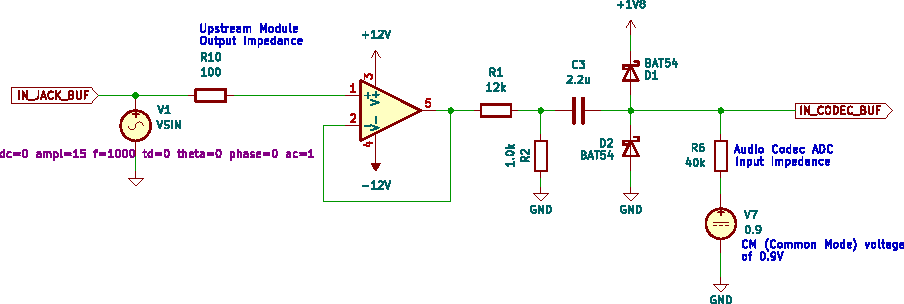
\includegraphics[width=0.8\textwidth]{../images/hardware_design/simulation/schem_audio_in_stage_simulation.pdf}
	\caption{Input stage schematic: unity-gain buffer followed by passive voltage divider.}
	\label{fig:schem_input_stage}
\end{figure}

\paragraph{Design Rationale}

The chosen signal-conditioning approach uses a unity-gain buffer followed by a passive resistor divider.
An inverting amplifier topology is unsuitable because its input impedance is fixed by the input resistor, making it impossible to simultaneously achieve the required high input impedance and the necessary attenuation without impractically large resistor values.
A non-inverting amplifier is unsuitable because its closed-loop gain
\[
A_\text{v} = 1 + \frac{R_\text{f}}{R_\text{g}} \geq 1
\]
cannot be less than unity, and therefore cannot attenuate the incoming signal.
The buffer followed by a passive divider avoids both limitations: the buffer presents a high impedance to the source, while the passive divider freely realises any attenuation factor below unity.
The divider consists of \(R_{1} = \qty{12}{\kilo\ohm}\) and \(R_\text{2} = \qty{1}{\kilo\ohm}\), giving an attenuation factor of
\[
a = \frac{R_\text{2}}{R_\text{1} + R_\text{2}} = \frac{1}{12} \approx 0,0833.
\]


\subparagraph{Input Stage Simulation}

A SPICE transient simulation was conducted to verify the input stage operating point with a \SI{10}{\volt_{pp}}, \qty{1000}{\hertz} input signal.

\begin{figure}[H]
	\centering
	\begin{minipage}{0.55\textwidth}
		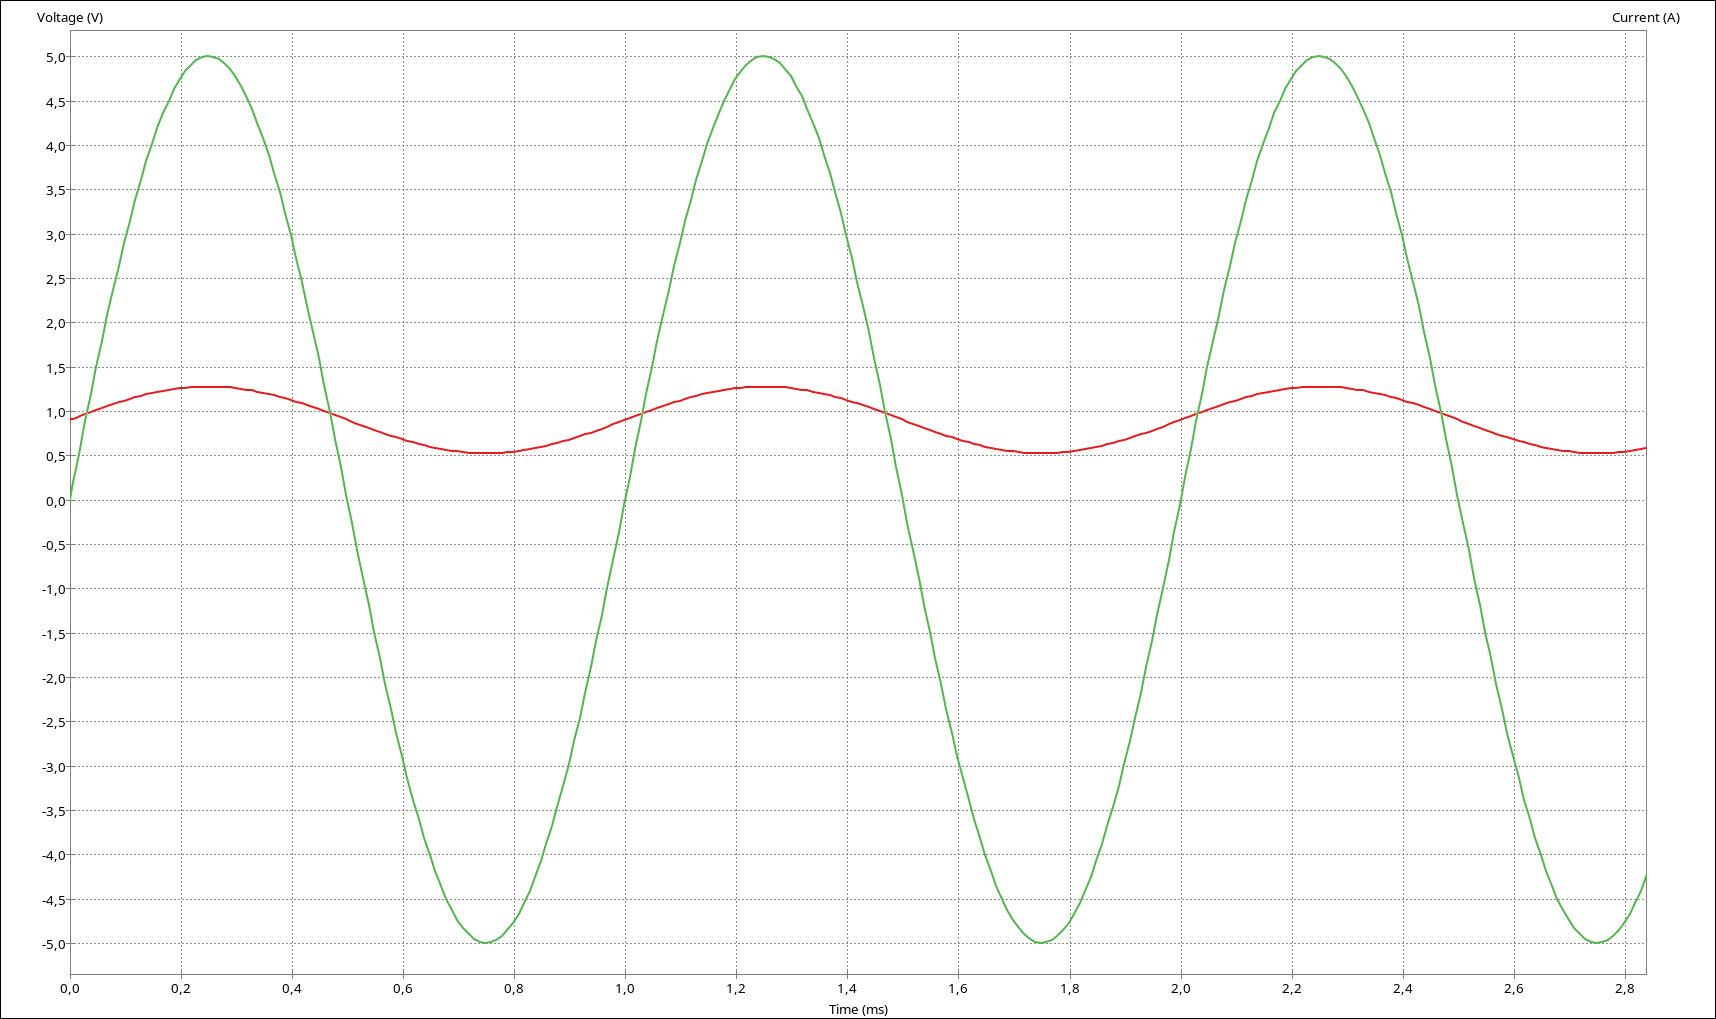
\includegraphics[width=\textwidth]{../images/hardware_design/simulation/trans_audio_in_simulation_print.png}
	\end{minipage}
	\hfill
	\begin{minipage}{0.30\textwidth}
		\centering
\begin{tabular}{lr}
	\toprule
 	\multicolumn{2}{l}{\textit{Source signal (Green)}} \\
	\multicolumn{2}{l}{\textit{V(IN\_JACK\_BUF)}} \\
	\midrule
	$V_\mathrm{pp}$  & \qty{10}{\volt} \\
	\midrule
	\multicolumn{2}{l}{\textit{Attenuated signal (Red)}} \\
	\multicolumn{2}{l}{\textit{V(IN\_CODEC\_BUF)}} \\
	\midrule
	$V_\mathrm{min}$ & \qty{523}{\milli\volt} \\
	$V_\mathrm{max}$ & \qty{1.28}{\volt}      \\
	$V_\mathrm{avg}$ & \qty{900}{\milli\volt} \\
	$V_\mathrm{pp}$  & \qty{752}{\milli\volt} \\
	\bottomrule
\end{tabular}
	\end{minipage}
	\caption{Transient simulation of the input stage with a \SI{10}{\volt_{pp}}, \qty{100}{\hertz} input signal.
		The attenuated output is centered at \qty{900}{\milli\volt} with a peak-to-peak amplitude of \qty{752}{\milli\volt}, within the ADC full-scale range of \SI{1.06}{\volt_{pp}}.}
	\label{fig:trans_input_stage}
\end{figure}

A Bode plot confirms the high-pass cutoff frequency of \qty{1.81}{\hertz} and the negligible phase shift across the audible range.

\begin{figure}[H]
	\centering
	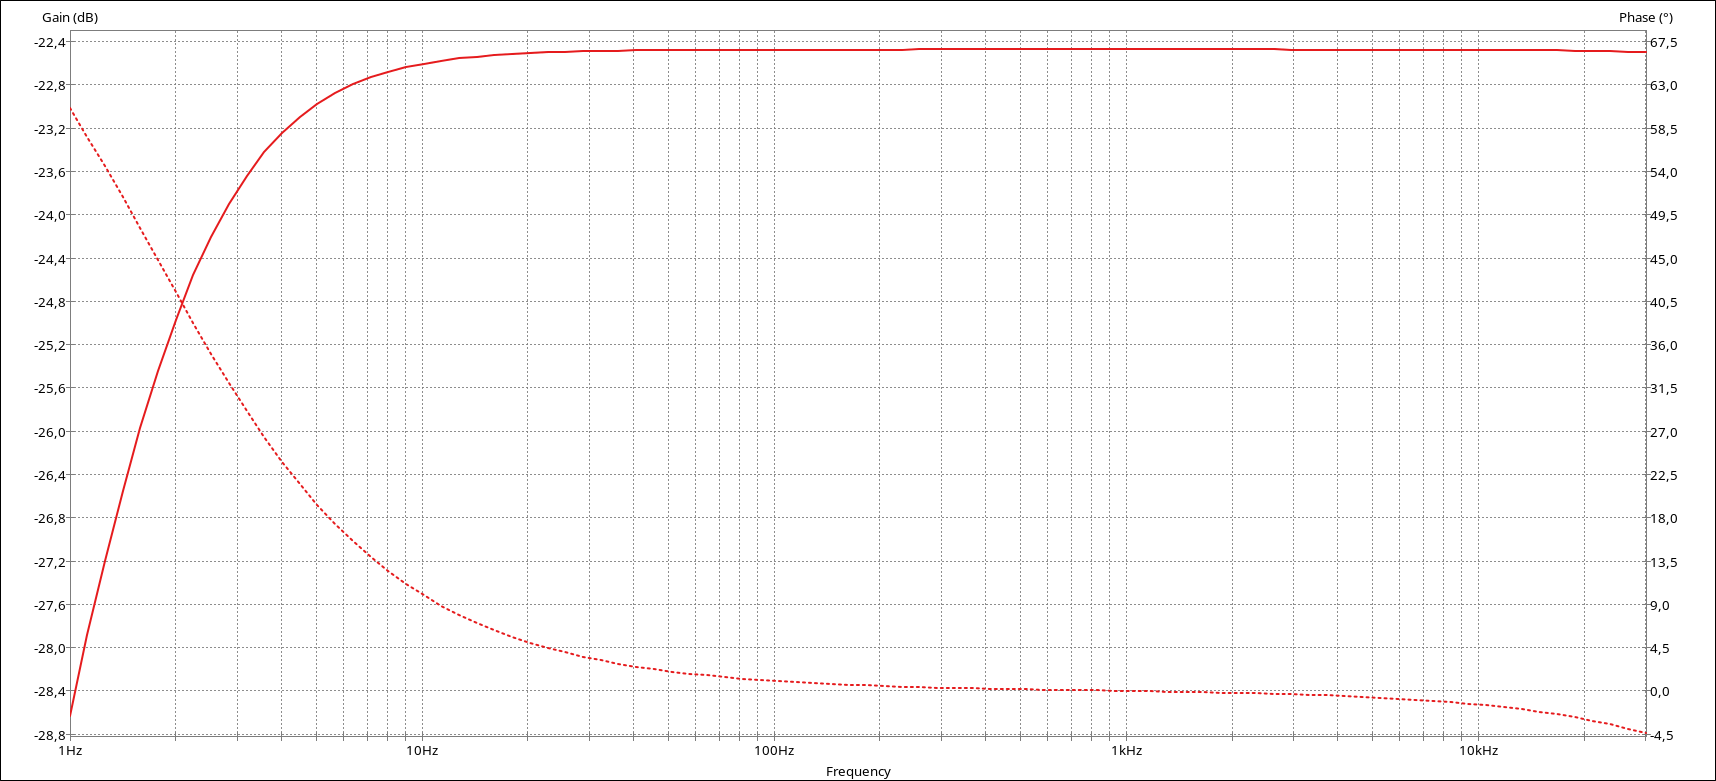
\includegraphics[width=0.8\textwidth]{../images/hardware_design/simulation/bode_audio_in_simulation_print.png}
	\caption{Bode plot of the input stage. The high-pass cutoff frequency of \qty{1.81}{\hertz} is well below the audible range, and phase shift remains negligible above \qty{20}{\hertz}.}
	\label{fig:bode_input_stage}
\end{figure}


\paragraph{Analog Output Stage Design}
\label{sec:output-ac-coupling}

\subparagraph{Design Rationale}

The DAC output signal is centered at a common-mode voltage of \(V_\mathrm{CM} = \SI{0.9}{\volt}\) with a maximum amplitude of \qty{0.7}{\volt}, which must be scaled up to the Eurorack line level of \qty{\pm 5}{\volt}.
An inverting op-amp topology is used, with \(R_8 = \qty{5.6}{\kilo\ohm}\) as the input resistor and \(R_9 = \qty{39}{\kilo\ohm}\) as the feedback resistor, yielding a closed-loop gain of
\[
A_v = -\frac{R_9}{R_8} = -\frac{39}{5.6} \approx -6.96.
\]
A coupling capacitor \(C_4 = \qty{10}{\micro\farad}\) is placed before \(R_8\) to strip the \qty{0.9}{\volt} DC offset from the DAC output.
Together with \(R_8\), this forms a high-pass filter with a cutoff frequency of
\[
f_c = \frac{1}{2\pi \cdot \qty{5.6}{\kilo\ohm} \cdot \qty{10}{\micro\farad}} \approx \qty{2.84}{\hertz},
\]
which is well below the audible range.
A \qty{1}{\kilo\ohm} series resistor at the op-amp output limits short-circuit current and isolates the amplifier from capacitive loads at the output jack.

\begin{figure}[H]
	\centering
	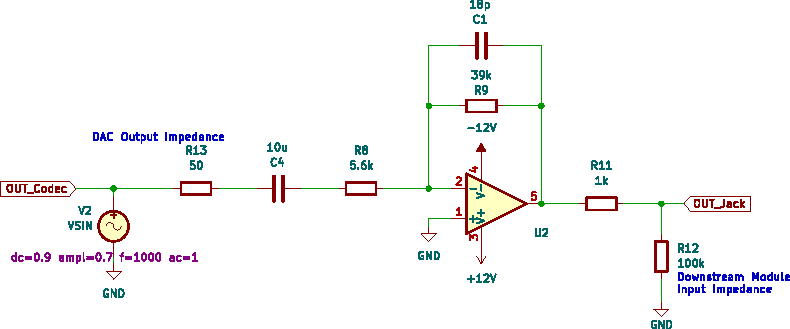
\includegraphics[width=0.8\textwidth]{../images/hardware_design/simulation/schem_audio_out_stage_simulation.pdf}
	\caption{Output stage schematic: AC-coupled inverting amplifier with current-limiting resistor.}
	\label{fig:schem_output_stage}
\end{figure}

\subparagraph{Output Stage Simulation}

A SPICE transient simulation was conducted to verify the output stage operating point.

\begin{figure}[H]
	\centering
	\begin{minipage}{0.65\textwidth}
		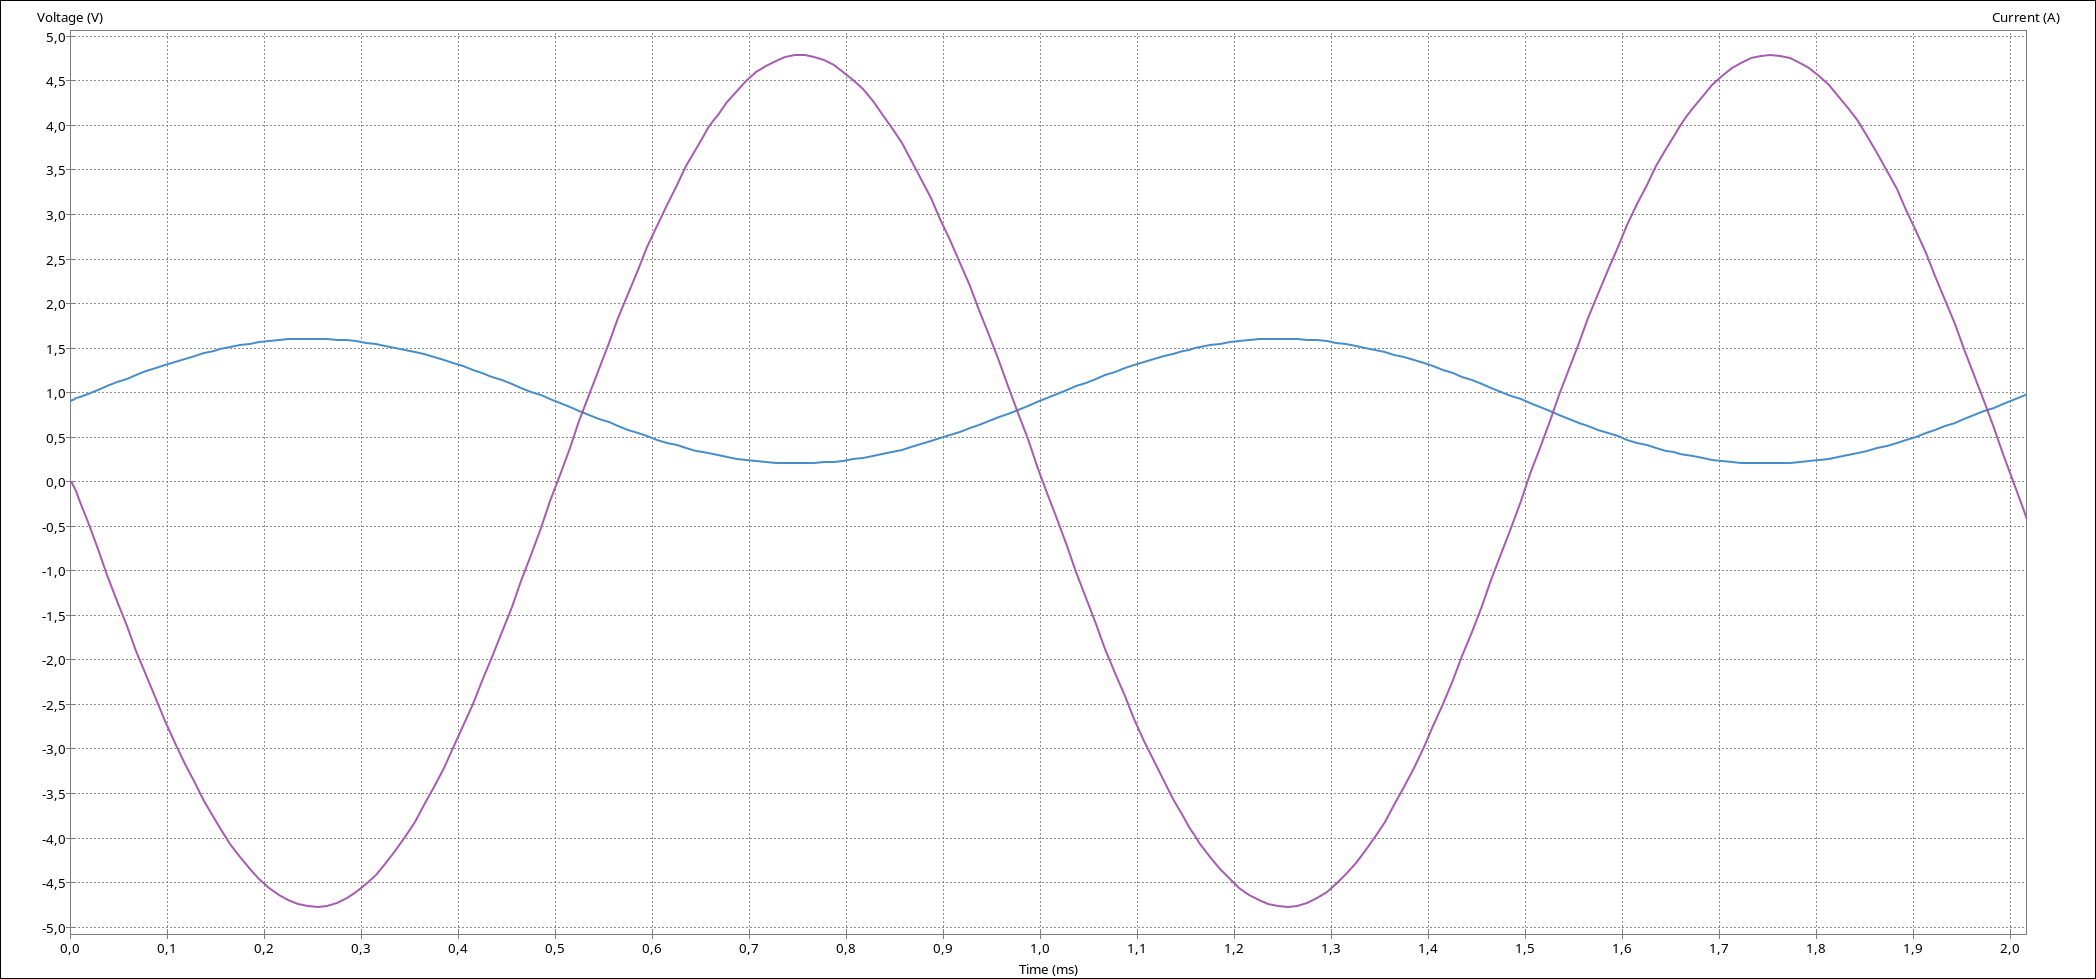
\includegraphics[width=\textwidth]{../images/hardware_design/simulation/trans_audio_out_simulation_print.png}
	\end{minipage}
	\hfill
	\begin{minipage}{0.30\textwidth}
		\centering
		\begin{tabular}{lr}
			\toprule
			\multicolumn{2}{l}{\textit{DAC output (Blue)}} \\
			\multicolumn{2}{l}{\textit{V(OUT\_Codec)}} \\
			\midrule
			$V_\mathrm{min}$ & \qty{200}{\milli\volt} \\
			$V_\mathrm{max}$ & \qty{1.60}{\volt}      \\
			$V_\mathrm{avg}$ & \qty{900}{\milli\volt} \\
			$V_\mathrm{pp}$  & \qty{1.40}{\volt}      \\
			\midrule
			\multicolumn{2}{l}{\textit{Jack output (Purple)}} \\
			\multicolumn{2}{l}{\textit{V(OUT\_Jack)}} \\
			\midrule
			$V_\mathrm{min}$ & \qty{-4.79}{\volt} \\
			$V_\mathrm{max}$ & \qty{4.78}{\volt}  \\
			$V_\mathrm{avg}$ & \qty{-5.43}{\milli\volt} \\
			$V_\mathrm{pp}$  & \qty{9.57}{\volt}  \\
			\bottomrule
		\end{tabular}
	\end{minipage}
	\caption{Transient simulation of the output stage. The DAC signal centered at \qty{900}{\milli\volt} is amplified and DC-decoupled to produce a \qty{9.57}{\volt_{pp}} output centered at \qty{0}{\volt}, within the Eurorack \qty{\pm 5}{\volt} specification.}
	\label{fig:trans_output_stage}
\end{figure}

A Bode plot confirms the high-pass cutoff frequency of \qty{2.84}{\hertz} and flat frequency response across the audible range.

\begin{figure}[H]
	\centering
	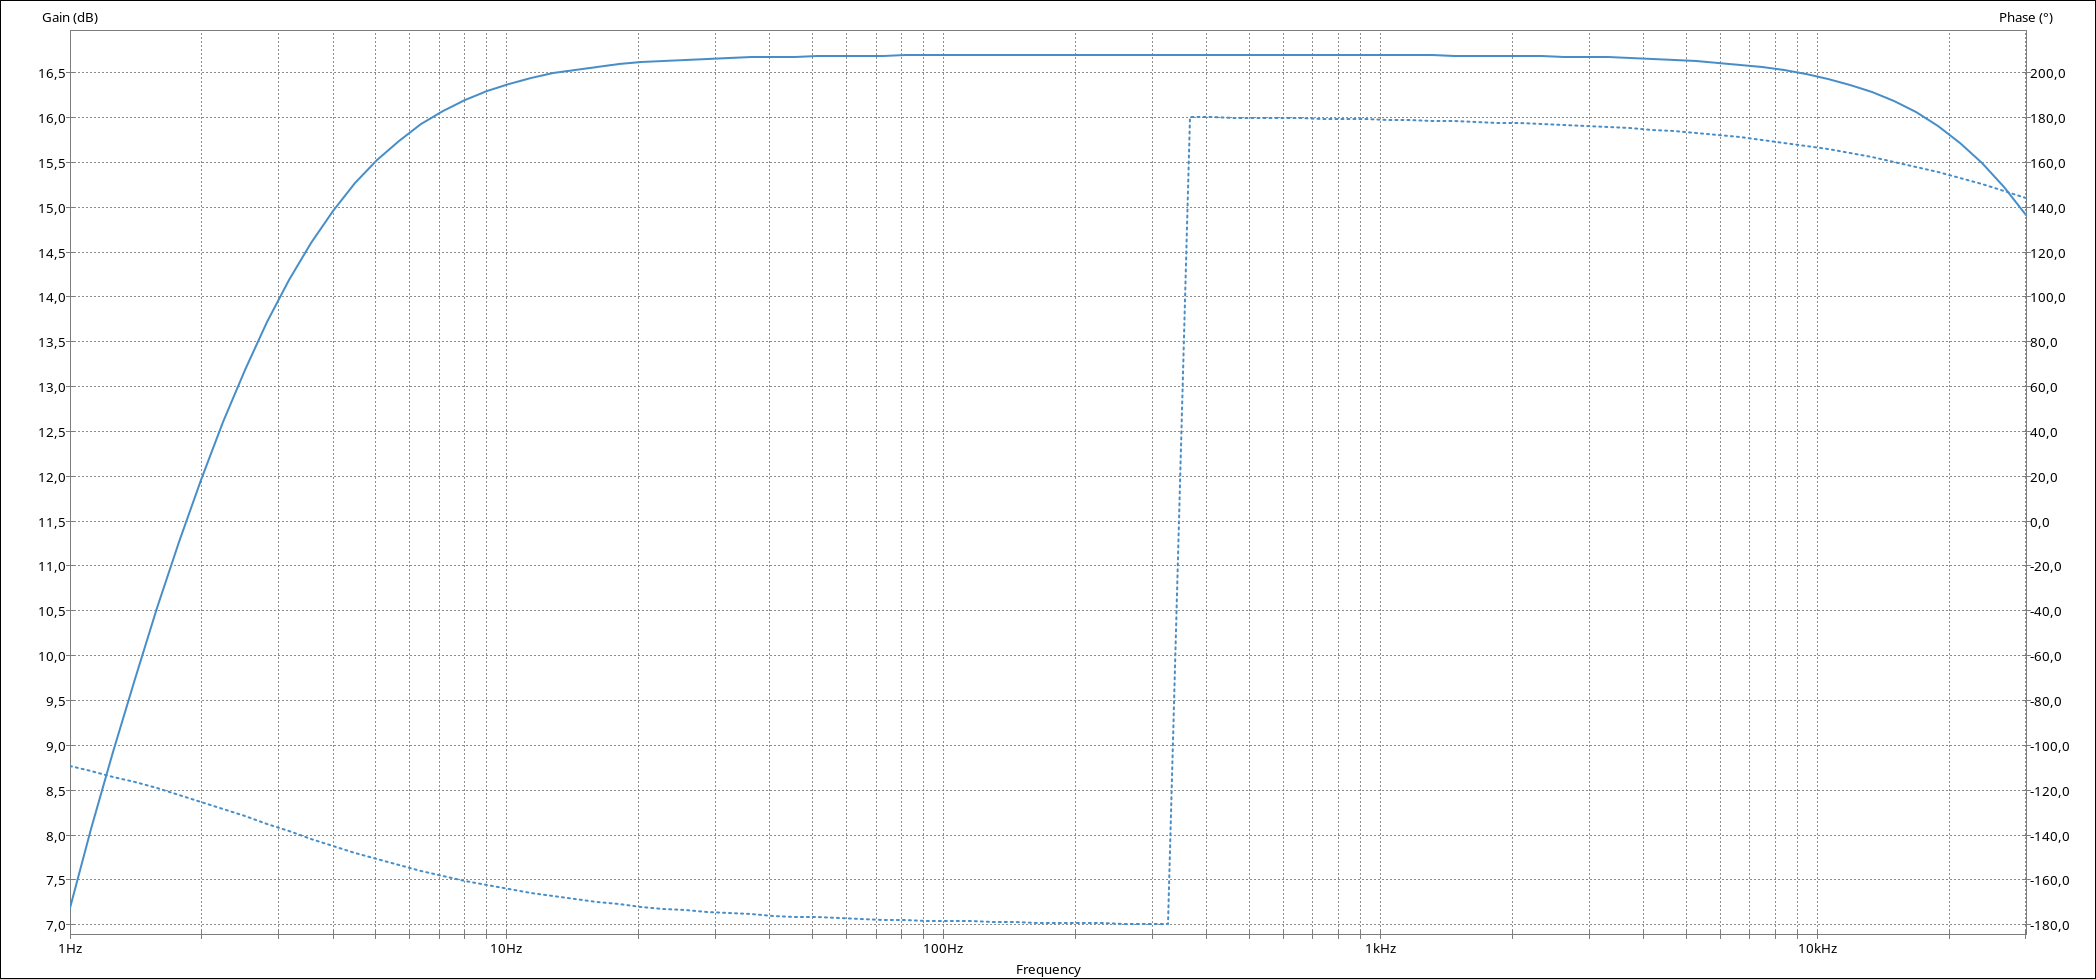
\includegraphics[width=0.75\textwidth]{../images/hardware_design/simulation/bode_audio_out_simulation_print.png}
	\caption{Bode plot of the output stage. The high-pass cutoff frequency of \qty{2.84}{\hertz} is well below the audible range, and the frequency response is flat up to \qty{20}{\kilo\hertz}.}
	\label{fig:bode_output_stage}
\end{figure}

\paragraph{CV Input Stage Design}
\label{ref:cv-input-stage-design}

\subparagraph{Design Rationale}

The CV input stages use an inverting summing amplifier topology, which differs from the audio input stage in two ways.
First, no AC coupling is used, as CV signals carry DC information that must be preserved.
Second, a bias resistor connected to a \qty{-10}{\volt} reference rail is summed at the inverting input to shift the output into the STM32H7 ADC input range of \qtyrange{0}{3.3}{\volt}.
This topology is derived from the CV input stage design used in the Mutable Instruments Clouds module \cite{pichenettesPichenettesEurorack2026}.

The general CV input accepts signals in the range of \qty{\pm 5}{\volt}, while the V/Oct input accepts \qty{-1.5}{\volt} to \qty{5}{\volt}.
Both circuits share the same topology with \(R_{in} = \qty{100}{\kilo\ohm}\), differing only in the bias and feedback resistor values to match their respective input ranges.
A \qty{1}{\nano\farad} capacitor in parallel with the feedback resistor acts as an anti-aliasing filter, attenuating high-frequency noise above the CV signal bandwidth.

\subparagraph{General CV Input}

For the general CV input, the bias resistor \(R_5 = \qty{200}{\kilo\ohm}\) is exactly twice the input resistor \(R_6 = \qty{100}{\kilo\ohm}\).
This means the \qty{-10}{\volt} reference contributes exactly half the weight of the input signal at the summing node, centering the output within the ADC range.
With feedback resistor \(R_7 = \qty{33}{\kilo\ohm}\), the output voltage is given by:
\[
V_{out} = -R_7 \left(\frac{V_{in}}{R_6} + \frac{\qty{-10}{\volt}}{R_5}\right)
= -33k \left(\frac{V_{in}}{100k} + \frac{-10}{200k}\right)
\]
At the input extremes:
\[
V_{out}(+5\,\text{V}) = \qty{0}{\volt}, \qquad V_{out}(-5\,\text{V}) = \qty{3.3}{\volt}
\]
mapping the full \qty{\pm 5}{\volt} CV range onto the \qtyrange{0}{3.3}{\volt} ADC input range.

\begin{figure}[H]
	\centering
	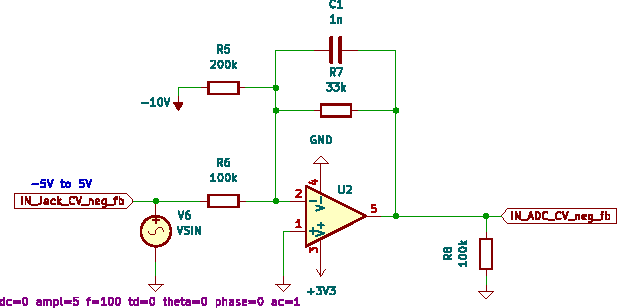
\includegraphics[width=0.65\textwidth]{../images/hardware_design/simulation/schem_cv_simulation.pdf}
	\caption{General CV input stage schematic: inverting summing amplifier with \qty{-10}{\volt} bias reference.}
	\label{fig:schem_cv_input}
\end{figure}

\subparagraph{V/Oct Input}

The V/Oct input covers the range \qty{-1.5}{\volt} to \qty{5}{\volt}, corresponding to a standard one-octave-per-volt keyboard range.
The bias and feedback resistors are adjusted to \(R_9 = \qty{180}{\kilo\ohm}\) and \(R_{11} = \qty{47}{\kilo\ohm}\) respectively, shifting and scaling the asymmetric input range onto the ADC window.

\begin{figure}[H]
	\centering
	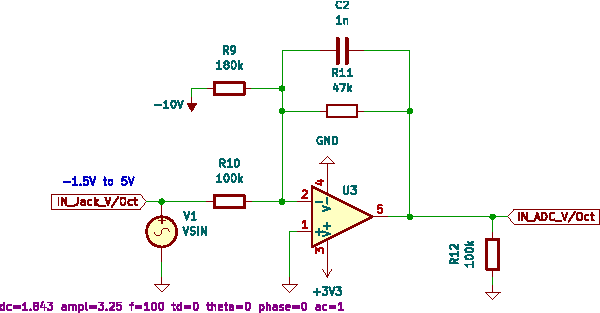
\includegraphics[width=0.65\textwidth]{../images/hardware_design/simulation/schem_voct_simulation.pdf}
	\caption{V/Oct input stage schematic: inverting summing amplifier with \qty{-10}{\volt} bias reference, dimensioned for the V/Oct input range.}
	\label{fig:schem_voct_input}
\end{figure}

\subparagraph{CV Input Stage Simulation}

Transient simulations were conducted for both CV input channels to verify correct level shifting and scaling into the STM32H7 ADC input range of \qtyrange{0}{3.3}{\volt}.

\begin{figure}[H]
	\centering
	\begin{minipage}{0.55\textwidth}
		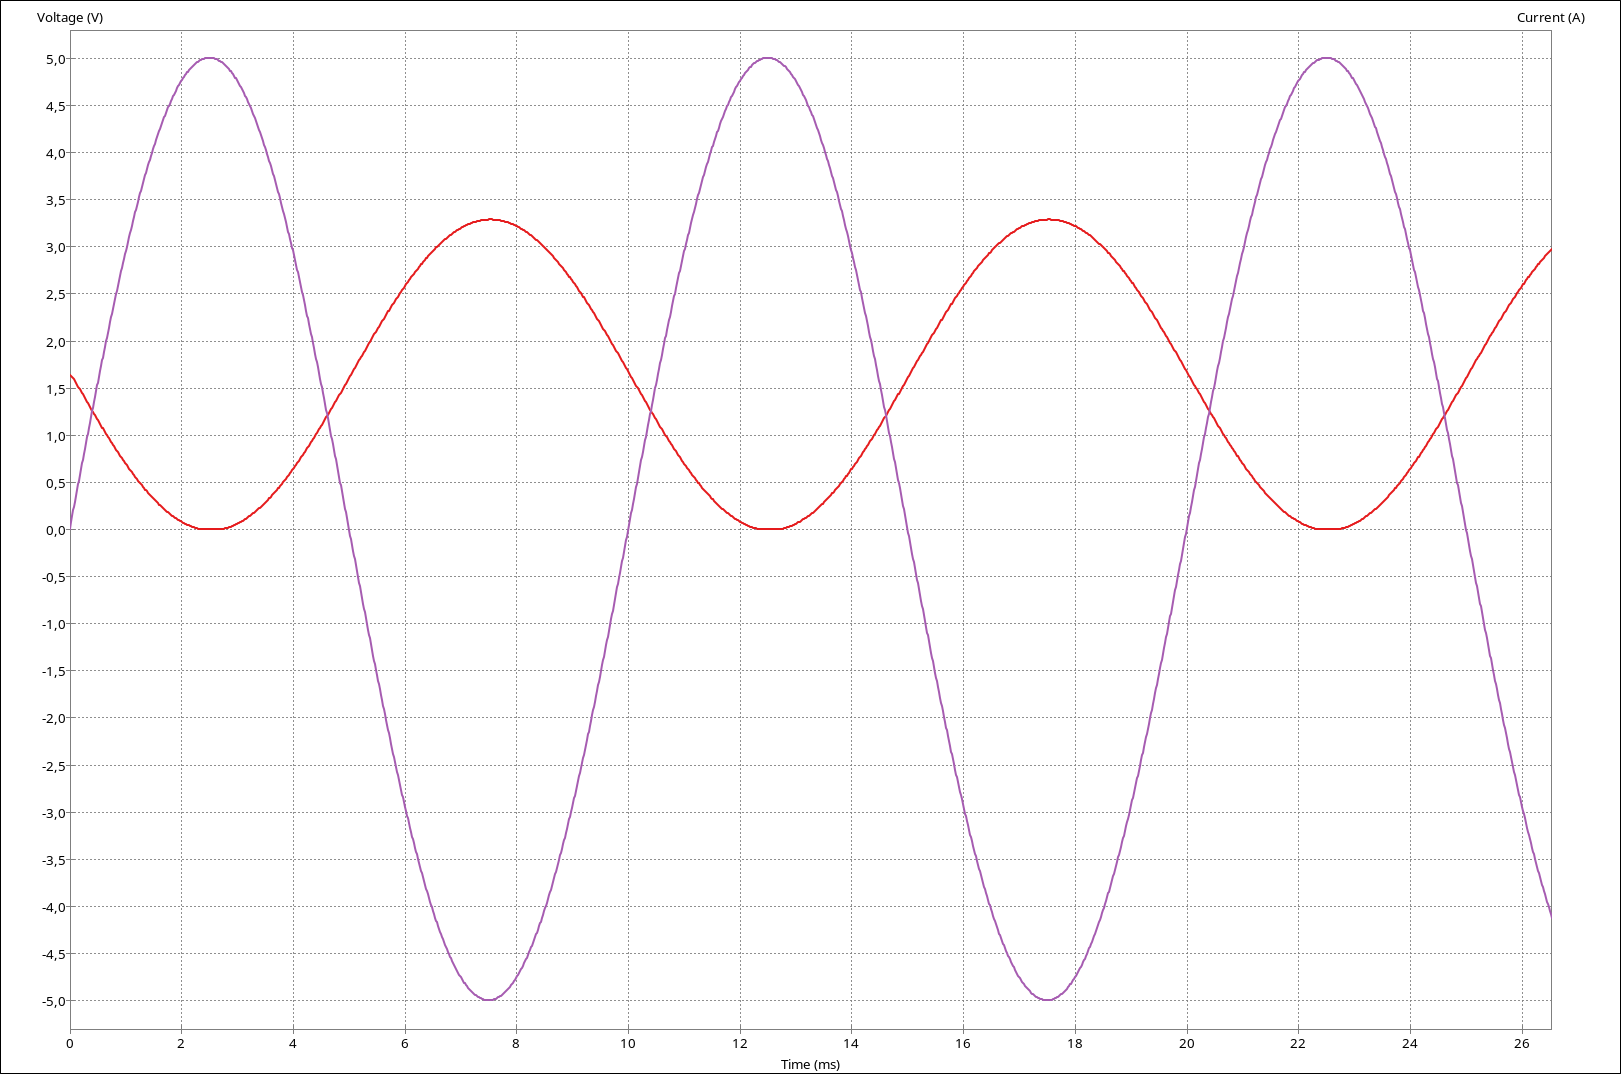
\includegraphics[width=\textwidth]{../images/hardware_design/simulation/trans_cv_simulation_print.png}
	\end{minipage}
	\hfill
	\begin{minipage}{0.30\textwidth}
		\centering
		\begin{tabular}{lr}
			\toprule
			\multicolumn{2}{l}{\textit{Source signal (Purple)}} \\
			\multicolumn{2}{l}{\textit{V(IN\_Jack\_CV)}} \\
			\midrule
			$V_\mathrm{pp}$  & \qty{10}{\volt} \\
			\midrule
			\multicolumn{2}{l}{\textit{ADC signal (Red)}} \\
			\multicolumn{2}{l}{\textit{V(IN\_ADC\_CV)}} \\
			\midrule
			$V_\mathrm{min}$ & \qty{-4.66}{\milli\volt} \\
			$V_\mathrm{max}$ & \qty{3.28}{\volt} \\
			$V_\mathrm{avg}$ & \qty{1.64}{\volt} \\
			$V_\mathrm{pp}$  & \qty{3.29}{\volt} \\
			\bottomrule
		\end{tabular}
	\end{minipage}
	\caption{Transient simulation of the general CV input stage with a \SI{10}{\volt_{pp}}, \qty{100}{\hertz} input signal.
		The output is centered at \qty{1.64}{\volt} and spans \qtyrange{0}{3.28}{\volt}, covering the full STM32H7 ADC input range.}
	\label{fig:trans_cv_input}
\end{figure}

\begin{figure}[H]
	\centering
	\begin{minipage}{0.55\textwidth}
		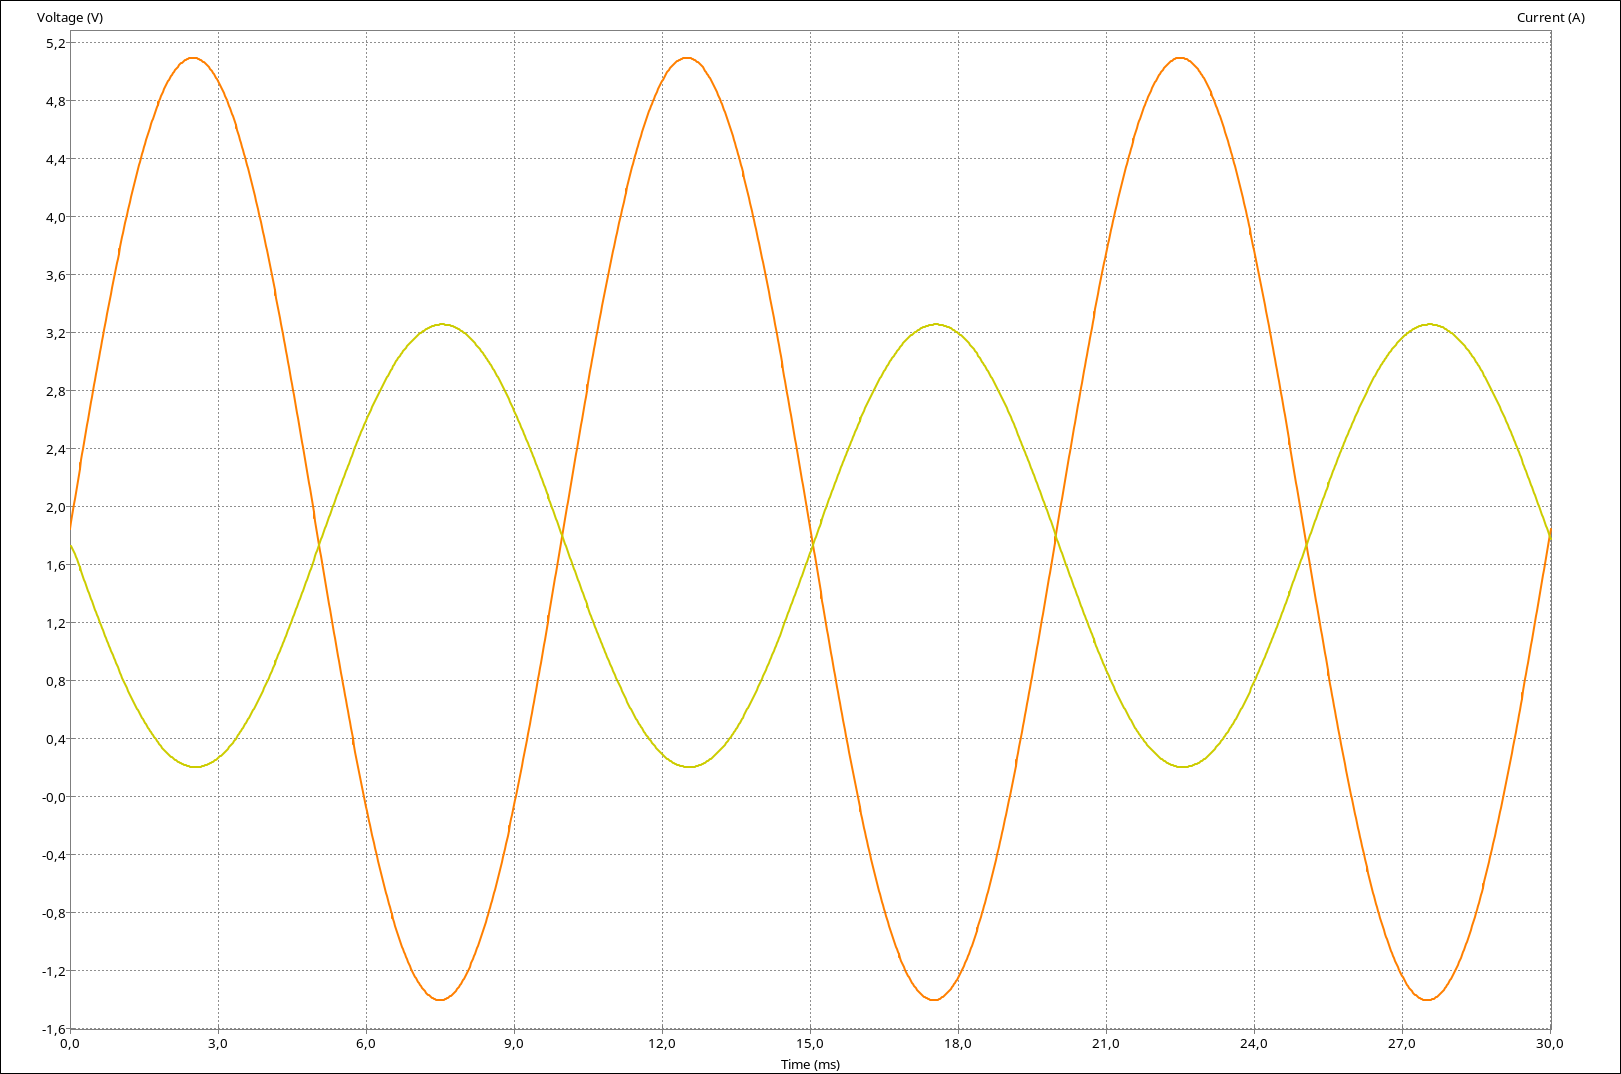
\includegraphics[width=\textwidth]{../images/hardware_design/simulation/trans_v_oct_simulation_print.png}
	\end{minipage}
	\hfill
	\begin{minipage}{0.30\textwidth}
		\centering
		\begin{tabular}{lr}
			\toprule
			\multicolumn{2}{l}{\textit{Source signal (Orange)}} \\
			\multicolumn{2}{l}{\textit{V(IN\_Jack\_V/Oct)}} \\
			\midrule
			$V_\mathrm{min}$ & \qty{-1.41}{\volt} \\
			$V_\mathrm{max}$ & \qty{5.09}{\volt} \\
			$V_\mathrm{pp}$  & \qty{6.50}{\volt} \\
			\midrule
			\multicolumn{2}{l}{\textit{ADC signal (Yellow)}} \\
			\multicolumn{2}{l}{\textit{V(IN\_ADC\_V/Oct)}} \\
			\midrule
			$V_\mathrm{min}$ & \qty{201}{\milli\volt} \\
			$V_\mathrm{max}$ & \qty{3.25}{\volt} \\
			$V_\mathrm{avg}$ & \qty{1.73}{\volt} \\
			$V_\mathrm{pp}$  & \qty{3.05}{\volt} \\
			\bottomrule
		\end{tabular}
	\end{minipage}
	\caption{Transient simulation of the V/Oct input stage with a \qty{-1.5}{\volt} to \qty{5}{\volt} input signal.
		The output spans \qty{201}{\milli\volt} to \qty{3.25}{\volt}, fitting within the STM32H7 ADC input range.}
	\label{fig:trans_voct_input}
\end{figure}